La resistenza ai guasti è uno dei parametri di valutazione di un sistema distribuito. Più è alto il numero dei nodi partecipanti (e dunque collegamenti), più è alta la probabilità di malfunzionamenti. Ad esempio è possibile avere ritardi, crash dei processi e nodi compromessi/malevoli. Questi malfunzionamenti vengono chiamati partial failure nel sistema. Un buon sistema distribuito fornisce trasparenza (in questo caso rispetto ai guasti) ovvero deve ovviare al malfunzionamento senza che l'utente possa percepirne gli effetti. \\

La \textit{Fault tollerance} è collegata alla \textit{dependability}, la quale implica:
\begin{itemize}
    \item disponibilità: probabilità che il sistema operi correttamente in ogni singolo istante
    \item affidabilità: il sistema deve riuscire a rimanere attivo (senza guasti) il più a lungo possibile
    \item safety: nel caso in cui ci fosse un guasto, questo deve essere gestito in modo tale che non si blocchi l'intero sistema. Bisogna dunque replicare le risorse affinchè questi guasti non portino ad eventi catastrofici
    \item maintaniblity: abilità di riparare facilmente un sistema che ha fallito o ha dei malfunzionamenti
\end{itemize}

Un aspetto importante è che un sistema può avere alta \textit{disponibilità}, ma bassa \textit{affidabilità}: il sistema risulta dunque quasi sempre disponibile, ma rimane inattivo per pochissimo tempo con una certa frequenza. Può anche avere alta \textit{affidabilità}, ma bassa \textit{disponibilità}. Quello che si cerca di ottenere è dunque un buon comportamento sotto entrambi gli aspetti.

\newpage
\section{Modelli di fallimento}
Ci possono essere vari modelli di fallimento all'interno del sistema:
\begin{itemize}
    \item crash failure: un server (nodo del sistema) che funziona perfettamente smette di funzionare
    \item omission failure: problemi nel ricevere e/o inviare messaggi 
    \item timing failure: la risposta del server non rientra nel timeout
    \item response failure: il valore di una risposta non è quello che ci si aspetta oppure il flusso di controllo di un nodo non segue quello previsto
    \item arbitrary failure: un server potrebbe produrre risposte arbitrarie in momenti arbitrari. Rientra in questo failure anche il Byzantine failure nel quale dei server devono mettersi d'accordo su qualcosa e per via dei ritardi delle risposte e/o dei fallimenti i server potrebbero non riuscire ad arrivare ad uno stato di consenso 
\end{itemize}

\subsection{Mascheramento dei guasti per ridondanza}
Per rendere più robusto un sistema rispetto ai guasti, il primo intervento che si utilizza (non solo in ambito di algoritmi) è aumentare i componenti. Un esempio è avere un server di riserva

\begin{itemize}
    \item Information redundancy: si usano dei bit per cercare di ricostruire il messaggio quando c'è del rumore presente
    \item Time redundancy: se una transazione viene abortita, può essere ripetuta. L'utente finale vede un po' di ritardo, ma riesce comunque ad ottenere la risorsa
    \item Physical redundancy: hardware o processi in più al fine di sopperire al mal funzionamento di qualche componente
\end{itemize}
\phantom \\

ESEMPIO:\\
Abbiamo un circuito con 3 dispositivi che si passano il segnale in sequenza. Se uno di questi funziona male, c'è un'alta possibilità che il circuito dia un risultato scorretto.
Uno dei modi è replicarli. Replichiamo quindi A, B e C con altre due copie.
Introduciamo dei componenti nuovi come il voter il quae emette un segnale se lo riceve in input dalla maggioranza dei dispositivi ad esso collegato. Se una delle 3 malfunziona, il voter da come output il valore dei due funzionano bene. Anch'essi non sono totalmente affidabili, dunque c'è ridondanza anche sui voter. Un failure tollerato per ogni componente (A, B e C)

\begin{center}
    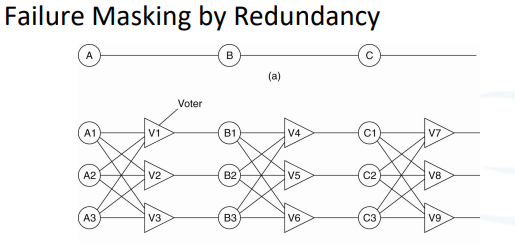
\includegraphics[width = 1\textwidth]{images/lezione5/fmr.png}
\end{center}

\subsection{Process resiliance}
Il Process resiliance è possibile dedurlo da ciò che è stato fatto nell'ambito dell'hardware. Possiamo gestire la ridondanza usando gruppi di processi, invece che un singolo processo. Ogni processo riceve i messaggi del gruppo e per fare ciò è necessario un protocollo/meccanismo per fare il join/leave del gruppo. Quanta ridondanza abbiamo bisogno? Dipende dai tipi di guasti:

\begin{itemize}
    \item crash: il client fa una richiesta al server. Se il server fallisce, il sistema è bloccato. Se abbiamo due processi nel gruppo e uno solo va in crash, l'altro è sufficiente per mascherare il malfunzionamento. Basta che resti attivo un processo nel gruppo per restituire il valore al client. Basta che resti attivo un processo nel gruppo per restituire il valore al client. Se invece, più processi rimangono attivi, restituiranno lo stesso valore al client. Il client gestirà  queste risposte tutte uguali e riesce lui a fare da voter. K+1 processi forniscono k fault tolerance
    \item wrong values: se consideriamo il caso in cui i processi nel gruppo possano dare risposte al client con valori sbagliati, per garantire k fault-tolerance necessitiamo almeno 2k + 1 processi nel gruppo
\end{itemize}


\subsection{Problemi di accordo}
Il consenso è una proprietà in cui si vuole che i processi di un certo gruppo si mettano d'accordo sul valore di un certa variabile. Questi problemi di accordo si chiamano: \textit{agreement problems}. Un esempio di questi problemi è riscontrabile andando ad analizzare lo stato di una macchina: finchè lo stato corrisponde ad un singolo nodo è chiaro, ma se la macchina è l'immagine di un gruppo di processi nel sistema distribuito, bisogna che tutti i nodi siano d'accordo su quale sia lo stato effettivo della macchina. E' dunque necessario che ogni nodo abbia la stessa informazione e questa deve essere mantenuta consistente.
Tra gli agreement problems si trovano:

\begin{itemize}
    \item consenso: ciascun processo propone un valore e i processi che non sono malfunzionanti dovrebbero mettersi d'accordo su un unico valore
    \item generali bizantini: un processo (commander) propone un valore e tutti gli altri processi devono concordare su questo valore. Anche il comandante potrebbe non dare il valore giusto duqnue tutti i partecipanti devono mettersi d'accordo e il valore corretto dev'essere uno. Se il comandante non è faulty, tutti devono concordare
    \item interactive consistency: ogni processo propone un valore e tutti i processi non faulty concordano su un vettore di valori (che contiene cosa ha detto ciascuno). Se ci sono processi che fanno apposta a confondere, occorre che quelli non malevoli capiscano cosa hanno detto tutti quelli non malevoli

\end{itemize}

\phantom \\

Ognuno di questi problemi risulta molto complesso e a volte anche irrisolvibile. Se si ha una soluzione per uno di questi problemi, è abbastanza facile usare la stessa soluzione per risolvere gli altri due.

\subsubsection{Risultato dell'accordo bizantino con sistemi sincroni}
Nel caso di agreement con malfunzionamenti bizantini servono almeno N = 3k + 1 processi per riuscire ad arrivare al consenso e ottenere k-fault tollerance. Questo vale per sistemi sincroni. Sotto certe assunzioni, si riesce dunque a risolvere il problema.
\newline
\newline
\textbf{Esempio di soluzione per il problema dei generali bizantini per N = 4 e k = 1:} 
\begin{itemize}
    \item Il comandante (uno dei quattro) manda un valore agli altri 3. Ognuno dei 3 manda il valore che ha ricevuto agli altri peer. Nel caso di 4 bastano 2 cicli di questo algoritmo. Nel caso di più di 4, va avanti: chi riceve i messaggi dei peer a sua volta manda il messaggio che ha ricevuto con un numero di round dipendente da N. Nel primo esempio, p2 e p4 ricevono una maggioranza di v. Nel secondo esempio, nessuno dei 3 riceve una maggioranza e l'algoritmo utilizza, quindi, un carattere speciale che è indeterminato, che è impossibile che sia uguale a quello del comandante e riconoscono che il comandante non è affidabile. Dovranno quindi provvedere ad eleggere un nuovo comandante e ripetere il processo.
\end{itemize}

\begin{center}
    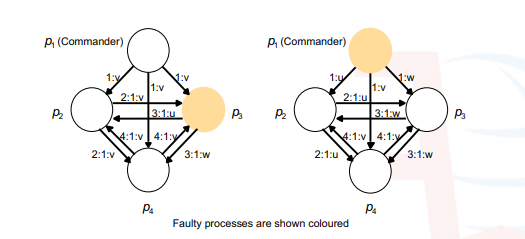
\includegraphics[width = 1\textwidth]{images/lezione5/bizantini.png}
\end{center}

\section{Sistemi sincroni VS sistemi asincroni}
I nodi all'interno di un sistema distribuito si scambiano messaggi affinché emerga una condivisione di valori tra i processi che stanno funzionando correttamente. I sistemi si dividono in sistemi sincroni e asincroni:

\begin{itemize}
    \item Sincroni: nei sistemi sincroni si assume che l'esecuzione del codice su ogni nodo è limitata in termini di velocità e tempo. Anche i link di comunicazione hanno un delay di tramissione con un certo bound e il clock su ogni nodo può avere un drift rispetto all'utc che però è bounded, poiché ci sono meccanismi di sincronizzazione
    \item Asincroni: nei sistemi asincroni l'esecuzione su ogni nodo può avere velocità arbitraria, i link di comunicazione hanno diversi delay di trasmissione unbounded e il clock su ogni nodo può essere completamente disallineato
\end{itemize}

\phantom \\

I sistemi che usiamo nella realtà si avvicinano di più ai sistemi asincroni. Il problema è che il coordinamento e l'accordo nei sistemi asincroni è difficile e spesso impossibile. Di fatto molto spesso vengono fatte assunzioni di sincronicità parziale del sistema. E' dunque necessario utilizzare algoritmi che realizzano una forma di sincronizzazione anche se bisogna comunque tenere conto che tante soluzioni falliranno data la natura asincrona del sistema.

\newpage
\subsection{Impossibilità di accordo nei sistemi asincroni}
 
Teorema FLP (1985): Quando i ritardi nella risposta ai messaggi sono arbitrari non esiste una soluzione garantita per l'accordo bizantino (consenso in presenza di difetti bizantini). Questo significa che se c'è anche un solo nodo nel sistema che ha un comportamento bizantino e siamo nel caso estremo asincrono, quindi con assenza di garanzie, non c'è una soluzione perfetta al problema. Abbiamo dunque una sincronia parziale. (?)
\newline
\newline
Teorema CAP: Questo teorema afferma che è possibile garantire al massimo due (di tre) proprietà nel caso di r/w su memoria condivisa. Queste proprietà sono:
\begin{itemize}
    \item Consistenza: Ogni lettura riceve la scrittura più recente o un errore (implica che tutti i nodi vedano gli stessi dati)
    \item Disponibilità: Ogni richiesta riceve una risposta (sistema operativo in qualsiasi momento)
    \item Partition tolerance: Il sistema riesce a tollerare un numero arbitrario di messaggi persi (o ritardati)
\end{itemize}
\phantom \\

La partition tolerance accade spesso nei nostri sistemi, quindi la vogliamo. Questo implica che i sistemi reali devono rinunciare a uno degli altri due.

\subsection{Consenso pratico: il protocollo Paxos}
Questo protocollo è stato introdotto da Lamport nel 1989 e ad oggi ne esistono diverse versioni. Lo scopo di questo protocollo è risolvere il problema del consenso garantendo la consistenza in una rete di processi inaffidabili, che possono quindi guastarsi. \\
La versione base di questo protocollo, che comunque è complicatissima, non copre i failure bizantini. Questa versione tollera k-failing nodes avendo N = 2k+1.\\
Avendo Paxos molte versioni, ne esiste anche una per risolvere il problema bizantino. Dato che nel caso completamente asincrono non è possibile dare una soluzione completamente corretta, vengono fatte delle assunzioni. Anche se sono molto rare, esistono condizioni nelle quali questo algoritmo non riesce ad arrivare al suo obbiettivo. Questo algoritmo è alla base di molti tool moderni.

\newpage
\subsection{Consenso pratico: il protocollo Raft}
Il protocollo Raft nasce da un gruppo di ricerca di Stanford come soluzione alternativa e più semplice al protocollo Paxos.\\
Raft si pone due obiettivi:
\begin{itemize}
    \item Rendere più accessibile la comprensione del protocollo
    \item Rendere più facile l'implementazione e l'applicazione dell'algoritmo di consenso risetto a Paxos.
\end{itemize}
\phantom \\

Raft, come Paxos, ha lo scopo di trovare una soluzione alla distribuzione dello stato delle macchine e avere così un consenso sullo stato del sistema preservando la safety (consistenza). Una caratteristica fondamentale di Raft è che si basa sull'elezione di un leader e questo comporta tutta una serie di problematiche che sorgono nel caso in cui il leader si guasti. Raft non copre nè bizantine failures nè nodi malevoli, ma copre ritardo di messaggi e crash dei nodi. I nodi del sistema credono alla correttezza del leader eletto e 
tollera k nodi in errore con N = 2k + 1.










\begin{comment}


Ovviare al malfunzionamento senza che l'utente se ne renda conto.
Fault taulerance è fortemente correlata a dependability che implica:
- disponibilità: 
- affidabilità:
- sicurezza:
- manutenibilità: 

Modelli di fallimento:
GUARDA SLIDES

Mascheramento del fallimento con ridondanza
- ridondanza di informazione
- ridondanza di tempo
- ridondaza fisica

Resilienza di processo
....

Quanta ridondanza?

Agreement problems
- Consenso: ogni processo propone un valore singolo e i processi non-faulty devono accordarsi sullo stesso valore
- Byzantine generals problem: un processo (comandante) propone un valore v. Tutti i processi corretti devono accettare lo stesso valore. Se il comandando è non-faulty tutti accettano v.
- Interactive consistency: ogni processo propone un valore. Tutti i processi corretti accettano un vettore di valori che contiene tutti i valori proposti. 

Sistemi sincroni e asincroni:
....

Teorema CAP (DB distribuiti o WEb service dist): in un sistema asincrono è impossibile ottenere:
- Consistenza
- Disponibilità 
- Partition tolerance


_====---====_-==_-

Mara



Fault tolerance and consensus

La resistenza ai guasti è uno dei parametri di valutazione di un sistema distribuito. Più è alto il numero dei nodi partecipanti (e quindi collegamenti), più è alta la probabilità di malfunzionamento, in termini di ritardi, crash dei processi e nodi compromessi/malevoli. Questi malfunzionamenti vengono chiamati partial failure nel sistema. Un buon sistema distribuito fornisce trasparenza (in questo caso rispetto ai guasti, significa ovviare al malfunzionamento senza che l'utente possa percepirne gli effetti). 

Fault tollerance è collegata alla dependability, la quale implica:
- disponibilità, probabilità che il sistema operi correttamente in ogni singolo istante,
- affidabilità, up-time (tempo running senza problemi) lungo
- safety, anche se ci fosse un guasto occorre gestirlo in modo tale che non si blocchi tutto. Replicazione delle risorse per gestire questi guasti in modo che non porti ad eventi catastrofici.
- maintaniblity, abilità di riparare facilmente un sistema che ha fallito o ha dei malfunzionamenti.

Una cosa importante è che un sistema può avere alta availability, ma bassa reliability: sistema quasi sempre disponibile, ma rimane inattivo per pochissimo tempo con una certa frequenza. Può anche avere alta affidabilità, ma bassa disponibilità. Vogliamo avere un buon comportamento su entrambi i parametri.

Ci possono essere vari modelli di fallimento all'interno del sistema:
- crash failure, un server (nodo del sistema) smette di operare, ma fino a prima funzionava correttamente
- omission failure, problemi nel ricevere i messaggi che sono stati inviati oppure il server non manda i messaggi come invece avrebbe dovuto
- timing failure, la risposta del server non rientra nel timeout
- response failure, il valore di una risposta non è quello che ci si aspetta oppure il flusso di controllo di un nodo non segue quello previsto
- arbitrary failure, (bizantino) ???

Per rendere più robusto un sistema rispetto ai guasti, il primo intervento che si utilizza (non solo in ambito di algoritmi) è aumentare i componenti, avere quindi un server di riserva ad esempio.

Information redundancy: si usano dei bit per cercare di ricostruire il messaggio quando c'è del rumore presente
Ridondanza di tempo: se una transazione viene abortita, può essere ripetuta. L'utente finale vede un po' di ritardo, ma poi ha ciò che cercava, per ovviare a problemi di link
Ridodanza fisica: hardware o processi in più 

ESEMPIO:
Abbiamo un circuito con 3 dispositivi che si passano il segnale in sequenza. Se uno di questi funziona male, c'è un'alta possibilità che il circuito dia un risultato scorretto.
Uno dei modi è replicarli. Replichiamo quindi A, B e C con altre due copie.
Introduciamo dei componenti nuovi: voter, emette un segnale se lo riceve in input dalla maggioranza dei dispositivi ad esso collegato. Se una delle 3 malfunziona, il voter da come output il valore dei due funzionano bene. Anch'essi non sono totalmente affidabili, dunque c'è ridondanza anche sui voter. Un failure tollerato per ogni componente (A, B e C)

Process resiliance: si può dedurre da ciò che è stato fatto nell'ambito dell'hardware. Possiamo gestire la ridondanza usando gruppi di processi, invece che singolo processo. Ogni processo riceve i messaggi del gruppo e server un protocollo/meccanismo per fare il join/leave del gruppo. Quanta ridondanza abbiamo bisogno? Dipende dai tipi di guasti:
- crash: il client fa una richiesta al server. Se il server fallisce, il sistema è bloccato. Se abbiamo due processi nel gruppo e uno solo va in crash, l'altro è sufficiente per mascherare il malfunzionamento. Basta che resti attivo un processo nel gruppo per restituire il valore al client. Se invece, più processi rimangono attivi, restituiranno lo stesso valore al client. Il client gestirà  queste risposte tutte uguali e riesce lui a fare da voter. K+1 processi forniscono k fault tolerance. Se consideriamo il caso in cui i processi nel gruppo possano dare risposte al client con valori sbagliati, per garantire k fault-tolerance necessitiamo almeno 2k + 1 processi nel gruppo.

Il consenso è una proprietà in cui si vuole che i processi di un certo gruppo si mettano d'accordo sul valore di un certa variabile. Questi problemi di accordo si chiamano: agreement problems. Un esempio è quello dello stato di una macchina, che se è su un singolo nodo, è chiaro. Ma se questa macchin è l'immagine di un gruppo di processi nel sistema distribuito, bisogna che tutti siano d'accordo su qual è lo stato della macchina. Dobbiamo avere la stessa informazione nei diversi nodi, deve essere mantenuta consistente. Ci sono algoritmi per garantire questo.

- consenso: Ciascun processo propone un valore e i processi che non sono malfunzionanti dovrebbero essere tutti d'accordo su uno stesso valore. Ci sono diverse varianti di questo problema del consenso:
- generali bizantini: un processo (commander) propone un valore e tutti gli altri processi devono concordare su questo valore. Anche il comandante potrebbe non dare il valore giusto, tutti i partecipanti devono mettersi d'accordo e il valore corretto dev'essere uno. SE il comandante non è faulty, tutti devono concordare. 
- interactive consistency: ogni processo propone un valore e tutti i processi non faulty concordano su un vettore di valori (che contiene cosa ha detto ciascuno). Se ci sono processi che fanno apposta a confondere, occorre che quelli non malevoli capiscano cosa hanno detto tutti quelli non malevoli.

Questi problemi sono molto complessi ed in alcuni casi irrisolvibili. Se si ha una soluzione per uno di questi problemi, è abbastanza facile usare lo stesso algoritmo per risolvere gli altri due.

Nel caso di agreement con malfunzionamenti bizantini servono almeno N = 3k + 1 processi per riuscire ad arrivare al consenso e ottenere k-fault tollerance. Questo vale per sistemi sincroni. Sotto certe assunzioni, si riesce dunque a risolvere il problema.

Esempio: k=1 dobbiamo avere almeno 4 nodi. Il comandante (uno dei quattro) manda un valore agli altri 3. Ognuno dei 3 manda il valore che ha ricevuto agli altri peer. Nel caso di 4 bastano 2 cicli di questo algoritmo. Nel caso di più di 4, va avanti: chi riceve i messaggi dei peer a sua volta manda il messaggio che ha ricevuto con un numero di round dipendente da N. Nel primo esempio, p2 e p4 ricevono una maggioranza di v. Nel secondo esempio, nessuno dei 3 riceve una maggioranza e l'algoritmo utilizza, quindi, un carattere speciale che è indeterminato, che è impossibile che sia uguale a quello del comandante e riconoscono che il comandante non è affidabile. Dovranno quindi provvedere ad eleggere un nuovo comandante e quant'altro.

Ci sono diversi round in cui tutti spediscono agli altri per far in modo che attraverso questo scambio di messaggi riesca ad emergere una condivisione di valori tra i processi (?) che stanno funzionando correttamente. Questo funziona sotto determinate condizioni. Si dividono i sistemi in sincroni e asincroni.
Nei sistemi asincroni:
- si assume che l'esecuzione di codice su un certo nodo ha dei limiti di velocità e di tempo. Prima o poi la computazione va avanti.
- Anche i link di comunicazione hanno un delay di tramissione ocn un certo bound
- il clock su ogni nodo può avere un drift rispetto all'utc che però è bounded, poiché ci osno meccanismi di sincronizzazione

Asincroni:
- esecuzione su ogni nodo può avere velocità arbitraria
- link di comunicazione hanno diversi delay di trasmissione unbounded
- block su ogni nodo può essere completamente disallineato

I sistemi che usiamo nella realtà si avvicinano di più ai sistemi asincroni. Coordination e agreement fanno delle assunzioni di almeno parziale sincronismo nel sistema. Abbiamo bisogno di relaizzare la sincronizzazione, ma dobbiamo rasseggnarci al fatto che la realtà del sistema è asincrona. Dobbiamo quindi accettare che tante soluzioni falliscano.

Un altro dei risultati molto risultato nell'ambito dei sistemi distribuiti è il FLP theorem: se c'è un solo nodo nel sistema che ha comportamento bizantino e siamo nel caso estremo asincrono, quindi con assenza di garanzie, non c'è una soluzione perfetta al problema. 
... sincronia parziale ...

Un altro risultato è il CAP theorem (anchesso per sistemi asincroni): non è possibile avere un algoritmo che garantisca consistenza, disponibilità (attivo in ogni momento) e partition tolerance (una parte della rete può divenire isolata, avendo temporanee interruzioni tra parti della rete(?)), nel caso di r/w su memoria condivisa virtuale (?). Troviamo soluzioni che possono garantire al massimo due di queste. La partition tolerance accade spesso nei nostri sistemi, quindi la vogliamo. I sistemi reali devono rinunciare a uno degli altri due.

Esempi di sistemi reali fatti a lezione che scelgono uno piuttosto che l'altro

Protocollo Paxos: ne esistono molte versioni, si parla di una famiglia di protocolli. obbiettivo è risolvere problema del consenso in una rete di processi unreliable, che possono quindi guastarsi, garantendo la consistenza. La versione base di questo protocollo, che comunque è complicatissimo, non copre i failure bizantini. Tollera k failing nodes avendo N = 2k+1 sotto determinte assunzioni. C'è anche una versione di Paxos per risolvere il caso bizantino. Ci sono assunzioni perché nel caso completamente asincrono non è possibile dare una soluzione completamente corretta. Ci sono condizioni in cui questo algoritmo non riesce ad arrivare al suo obbiettivo, però sono molto rare. Sta alla base di molti tool moderni. Lamport parla del funzionamento del parlamento dell'isola di Paxos in cui i parlamentari entravano e uscivano liberamnete dal parlamento (?).

Per la difficoltà di questo protocollo, che però è ampiamente utilizzato, un gruppo di ricerca di Stanford ha fatto un nuovo protocollo che si chiama Raft.
Due obbiettivi: rendere più accessibile la comprensione del protocollo e rendere più facile l'implementazione e l'applicazione dell'algoritmo di consenso risetto a Paxos. obbiettivo è lo stesso: soluzione alla distribuzione dello stato delle macchine, avere consenso sullo stato del sistema preservando la safety (consistenza). Una caratteristica fondamentale è che si basa sull'elezione di un leader. Con tutte le problematiche del crash del leader. Raft non copre bizantine failures, copre ritardo di messaggi, crash dei nodi, ma non nodi malevoli. Gli altri nodi che non sono leader credono alla correttezza del leader. k tollerance con N = 2k+1




---------
Fabbio


Fault tolerance e consenso
Più è alto il numero di partecipanti e più alta è la probabilità che uno dei nodi e/o collegamenti presenti un malfunzionamento. I malfunzionamenti vengono identificati anche come partial failure nel sistema. 

Concetti base:
Concetti legati a sistemi che offrono "dependability". Termine che riflette la fiducia che un utente può avere nel sistema in termine di diverse cose:
-disponibilità: probabilità che il sistema operi correttamente in ogni istante
-reliability: l'abilità di funzoionare correttamente per molto tempo
-safety: i fallimenti non devono creare problemi catastrofici
-Mantenibilità: l'abilità di riparare facilmente un sistema che ha dei fallimenti.

Failure models: 

Process Relisience:
 

\end{comment}